%\begin{document}
% first step: page classification
\begin{frame}
\frametitle{Page Classification}
The first step:
\begin{itemize}
\item Separate the pages containing at least one image from those
containing none
\item Could serve as pre-processing step in annotating
\item Proof of concept
\end{itemize}
\end{frame}


% Briefly explain HOG features

\subsection{Method}

\begin{frame}
\frametitle{Features}
Local features to capture the difference between text and images:
	\begin{block}{Histogram of Oriented Gradients (HOG)}
		HOG features contain the amount of gradients in a certain image patch.
	\end{block}
	\begin{block}{Steps for computing HOG Features\cite{dalal2005histograms}}
	\begin{enumerate}
		\item Global image normalisation
		\item Compute the gradient images
		\item Compute gradient histograms in 8 directions
		\item Normalise across blocks
		\item Flatten into a feature vector
	\end{enumerate}
	\end{block}
\end{frame}

\begin{frame}[allowframebreaks]{HOG Examples}
	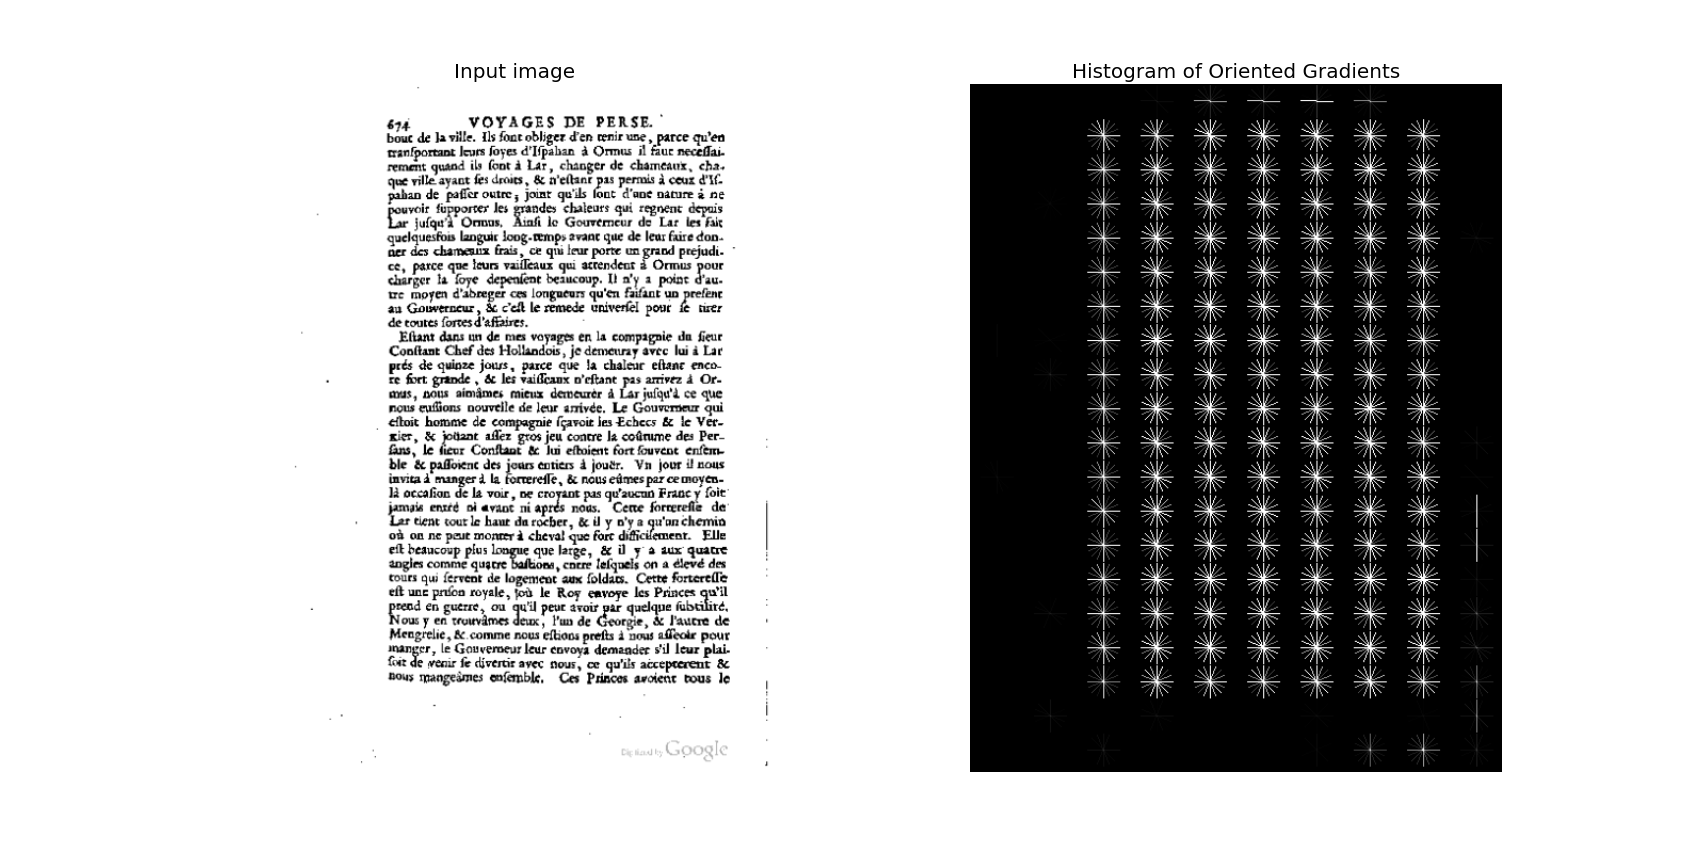
\includegraphics[trim=200px 0px 100px 0px, clip=true, width=.8\paperwidth]{resources/text1}\\
\framebreak
	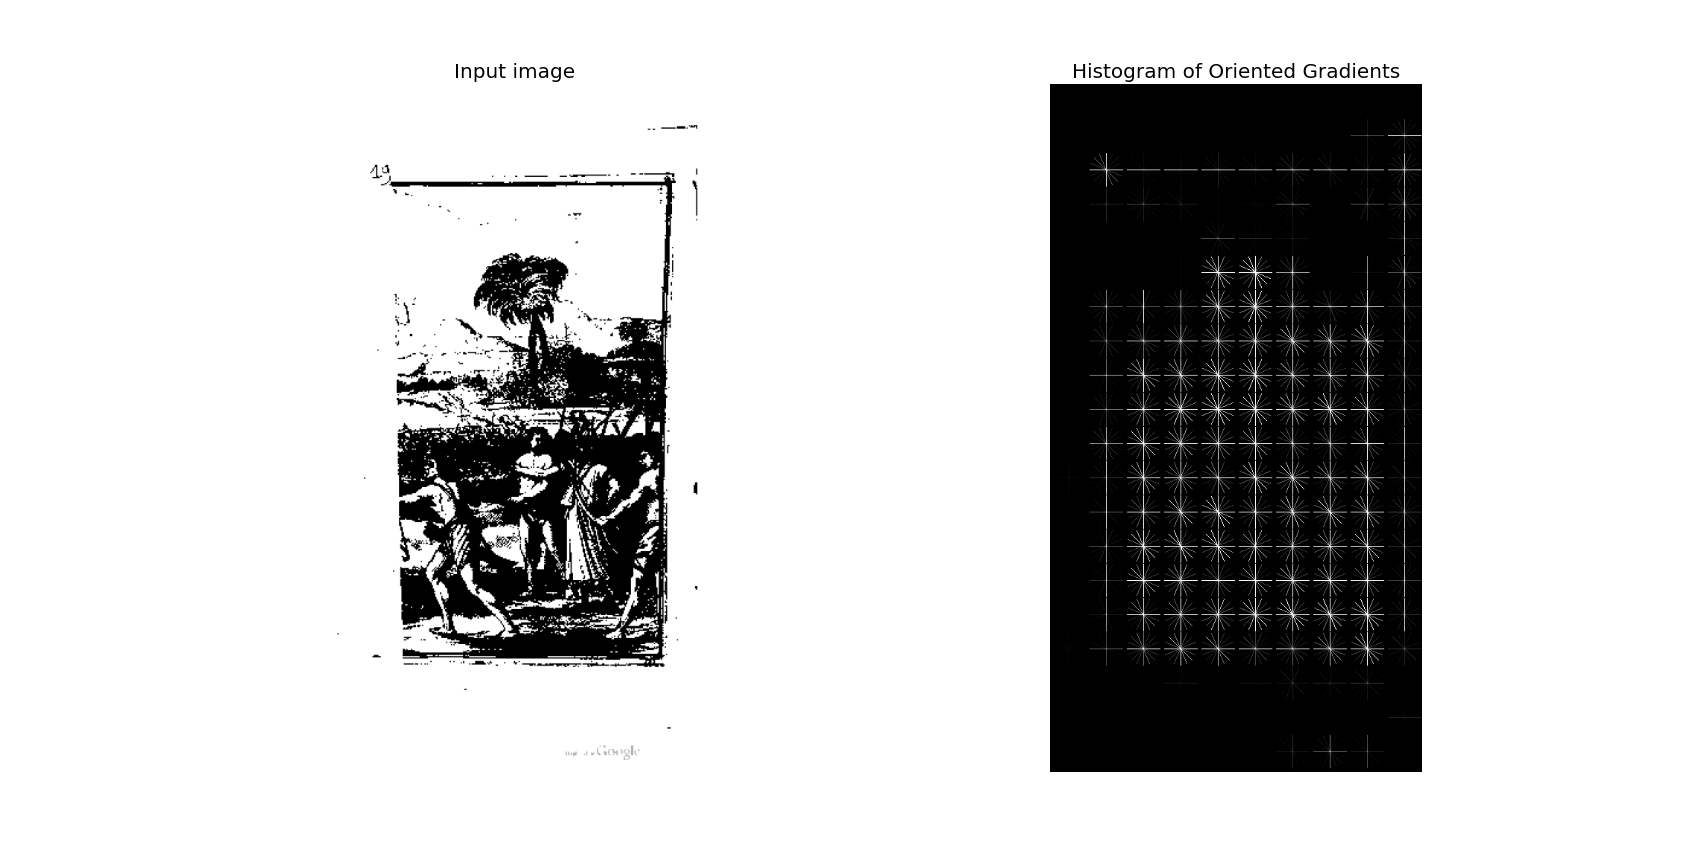
\includegraphics[trim=200px 0px 100px 0px, clip=true, width=.8\paperwidth]{resources/image1}\\
\framebreak
	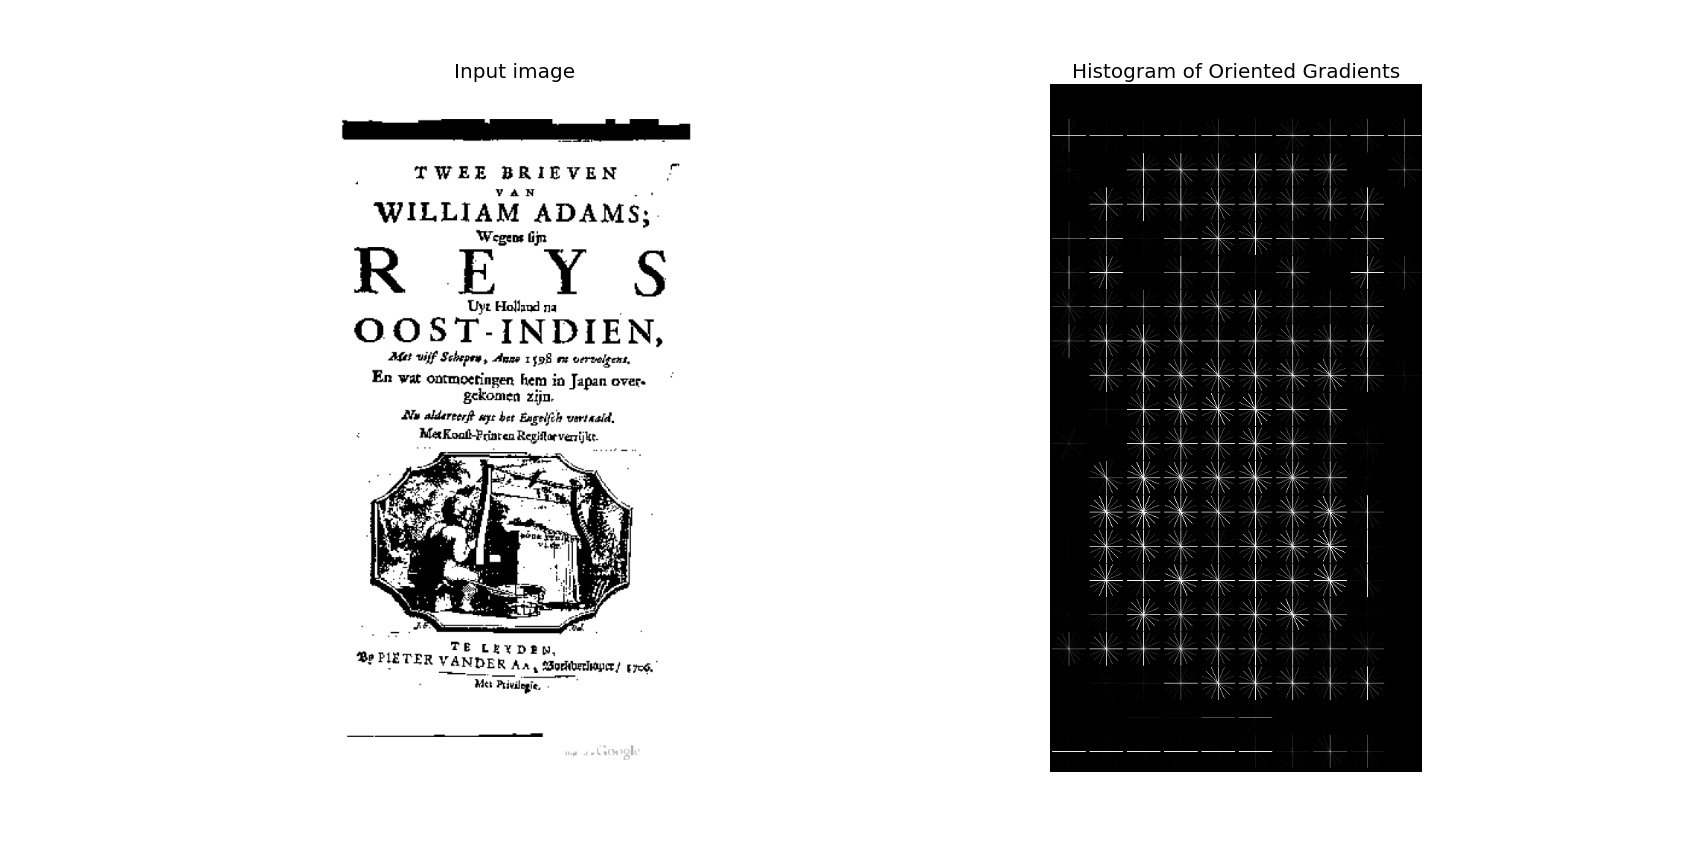
\includegraphics[trim=200px 0px 100px 0px, clip=true, width=.8\paperwidth]{resources/text_and_image1}
\end{frame}

% Explain SVM i.c.w. HOG features for pages
% Moved to introduction
% \slide{Classification using SVM}
% {
% 	\begin{itemize}
% 		\item All pages are annotated with having either ``text'', ``images'' or
% 		``nothing useful'' on it. Images get bounding boxes, which we will later
% 		use.
% 		\item Calculate 5x5 HOG features per page
% 		\item Train a Support Vector Machine (SVM) on these feature vectors and
% 		labels
% 		\item Predict whether a page contains an image based on this SVM
% 	\end{itemize}
% }

\begin{frame}
\frametitle{Train - Validation - Test}

\begin{block}{Train - Validation}
\begin{itemize}
\item Merge the sets of all annotated book pages into one set
\item Split this set into train set ($80\%$) and validation set($20\%$)
\item Use validation set to set parameters ($C$)
\item Use F2-score in order to focus on recall (preprocess for annotator)
\end{itemize}
\end{block}

\begin{block}{Test}
\begin{itemize}
\item Run the learned classifier on newly downloaded books
\end{itemize}
\end{block}
\end{frame}

\subsection{Results}
\begin{frame}
\frametitle{Results}

\begin{block}{Scores}
\begin{tabular}{l l l l}
% & \multicolumn{2}{c}{\emph{Pre-trained}} & \multicolumn{2}{c}{\emph{Direct}} \\
  & \textbf{Image} & \textbf{Text} & \textbf{Nothing} \\
\textbf{Precision} & 0.60  & 0.995 & 0.970 \\
\textbf{Recall} & 0.964  & 0.921 & 0.964 \\
\textbf{F-score} & 0.741 & 0.956 & 0.967
\end{tabular}
\end{block}

\begin{block}{Confusion matrix}
\begin{tabular}{l l l l}
%& \multicolumn{2}{c}{\emph{Pre-trained}} & \multicolumn{2}{c}{\emph{Direct}} \\
Real\textbackslash Predicted & \textbf{Nothing} & \textbf{Image} & \textbf{Text} \\
\textbf{Nothing} & 271 & 9 & 1 \\
\textbf{Image} & 169 & 2074 & 9 \\
\textbf{Text} & 10 & 2 & 323
\end{tabular}
\end{block}


%MET BAGGER
%[[ 271    9    1]
%[ 169 2074    9]
%[  10    2  323]]

%                       Precision:
%                               Image: 0.602222
%                               Text: 0.994724
%                               Bagger: 0.969970
%                       Recall:
%                               Image: 0.964413
%                               Text: 0.920959
%                               Bagger: 0.964179
%                       Fscore:
%                               Image: 0.741450
%                               Text: 0.956421
%                               Bagger: 0.967066
%                       Support:
%                               Image: 281.000000
%                               Text: 2252.000000
%                               Bagger: 335.000000
%


\end{frame}
